\chapter{Implementation} % Main chapter title

\label{Chapters} % For referencing this chapter elsewhere, use \ref{Chapters}

\lhead{Chapter 6. \emph{Implementation}}

%----------------------------------------------------------------------------------------
%	SECTION 6.1
%----------------------------------------------------------------------------------------

\section{Frame}

This section comes after the literature review and requirements analysis to present the frame the software implementation will be developed on. This section will first go through the motivations in the choice of the frame as well as some perspective to move away from the objective and cover what will not be issued.

%-----------------------------------
%	SUBSECTION 6.1.1 - Motivations
%-----------------------------------

\subsection{Motivations}

Two objectives were set by missing information from the literature review. First, whether it is for development or acceleration frameworks, few benchmarks compare a similar implementation implemented in different frameworks. In terms of acceleration frameworks, this is due to the fact that few of them have opened their source code, making it time-consuming for one to perform a correct benchmark of the different frameworks. The other objective is to assess the importance of quantisation. While it has been proven that \emph{QNNs} could achieve the same accuracy and better throughput than classic \emph{CNNs}, few effort has been put in assessing the benefits and finding the best tailored precision for one's application.

Very few benchmarks exist on existing technologies, whether it is on development frameworks, or acceleration frameworks. The presentation of an accelerator often differs a lot from associated works and only state-of-the-art networks accuracy and throughputs are compared on simple architectures. Few projects seem to grow from the article they emerged from. \emph{YodaNN} \cite{Andri2016} does not provide any code outside of the article, neither does \emph{F-CNN} \cite{Zhao2016}. \emph{Tomato} \cite{Zhao2019}, \emph{TinyCNN} \cite{Jahanshahi2019} and \emph{fpgaConvNet} \cite{Venieris2017} face the same issue and make any comparison between the different frameworks very time-consuming. Only \emph{FINN} \cite{Umuroglu2017a, Blott2018} is still in active development and open-source.

Setting a benchmark from the open-source acceleration framework can help any external user have both a direct implementation of the framework as well as backed-up arguments on why it can help deploy one's application, at what cost and compared to state-of-the-art implementation. While the first objective presented earlier would be too time-consuming to complete, the second one is made possible through the usage of the open-source accelerator.

The main motivations taken in consideration when setting up the \emph{Brevitas} / \emph{FINN} benchmark is to provide an insight on the Xilinx's tools and their workflow. This is important because widening the audience of the tool by presenting its capabilities allows both companies to be interested in the product as well as individuals to contribute to the project since it is open-source. The \emph{FINN} project started in September 2018 and has been in development ever since. The first version has been deprecated and a new direction is taken in 2019. The project is now using \emph{Brevitas}, a PyTorch extension to perform the training and quantisation. \emph{FINN} is aiming at providing a clear acceleration of inference by deploying a network on an FPGA board.

%--------------------------------------
%	SUBSECTION 6.1.2 - About Perspective
%--------------------------------------

\subsection{About Perspective}

% TODO ADD PAPERS THAT PROPOSE TRAINING ON FPGA
Several papers present methods to \emph{train} networks on FPGAs. However, while \emph{Brevitas} allows the training of \emph{QNNs}, it does not map the network on FPGAs at training time. It is expected to train the network on another hardware architecture (CPU(s) or GPU(s)) as PyTorch would expect and can handle. On the other hand, both \emph{Brevitas} and \emph{FINN} are in active development and in early phases of their development cycle. Version 0.3 of both tools has been released in late May this year.

%----------------------------------------------------------------------------------------
%	SECTION 6.2 - Workflow
%----------------------------------------------------------------------------------------

\section{Workflow}

This section will present the whole workflow \emph{Brevitas} / \emph{FINN} put into place. By first going through the \emph{QNN} designer and trainer that is \emph{Brevitas}, the quantised neural network is translated into the intermediate representation, \emph{ONNX}. The resulting intermediate representation can then be imported by \emph{FINN}. \emph{FINN} will perform several transformations and deploy part of the resulting graph on the associated FPGA.

%-----------------------------------
%	SUBSECTION 6.2.1 - Brevitas
%-----------------------------------

\subsection{Brevitas}

Brevitas has been developed with the idea of corresponding to a \guille{drop-in} replacement of PyTorch. This means that it ensures that PyTorch functionalities will be kept, even when working with reduced-precision layers. Brevitas implements a set of building blocks to model a reduced precision hardware data-path at training time. While partially biased towards modelling dataflow-style, very low-precision implementations, the building blocks can be parametrized and assembled together to target all sorts of reduced precision hardware.

The implementation sets up several design principles: idiomatic PyTorch if possible, modularity first at the cost of some verbosity and a focus on easy extendability. Brevitas features many different ideas such as extracted from its presentation:
\begin{itemize}
  \item \textbf{Quantisation Type}: Binary, ternary or uniform integer.
  \item \textbf{Target Tensor}: Weights, activations or accumulators.
  \item \textbf{Scaling}: Support for different shapes, learning strategies and constraints.
  \item \textbf{Precision}: Constant or learned bitwidth.
  \item \textbf{Cost}: Hardware cost modelled at training time.
\end{itemize}

Note that the \emph{scaling} is the method used by Brevitas to preserve a good precision even though the layers use quantised parameters. Brevitas handles several different methods to determine the scaling factor. It determines it either with respect to the number of dimensions, with respect to a learned parameter, shared between different layers or constrained to specific values. On the other hand, Brevitas supports both constant and learned precision.

As an example, we would like to define the \emph{LeNet-5} architecture as presented by Le Cun et al. \cite{LeCun1998}. The \emph{PyTorch} version can be seen on \emph{Figure} \ref{fig:LeNetPyTorch}. It consists of an extension of the \texttt{Module} class. The layers are then defined into two separate parts in the initialisation method. In one side and as part of a \texttt{Sequential}, the layers performing the \emph{feature extraction}. Those layers consist mostly of convolutions, pooling and activations, sometimes with batch normalisations and dropouts. In our case, the \emph{feature extraction} consists of three sequences of \texttt{Convolution => TanH Activation => Average Pooling}. Next comes the \emph{classifier} sequence, represented by a \texttt{Sequential} as well. It consists of fully-connected layers and end up with a number of neurons equal to the number of classes. Here, our \emph{classifier} consists of two fully-connected layers.

PyTorch asks to define the \texttt{function} and manages backpropagation on its own when dealing with a neural network. Here, the forward function consists of feeding the instance (image supposedly) in the \emph{feature extractor}, reshaping the result into a 1-dimensional array, feeding this array to the \emph{classifier} and using a \emph{softmax} function to access the probabilities determined for each of the classes of the dataset.

% PyTorch LeNet5 implementation
\begin{figure}[htbp]
\centering
\begin{lstlisting}[language=Python]
import torch
import torch.nn as nn
import torch.nn.functional as F

class LeNet5(nn.Module):
  '''LeNet5 architecture in PyTorch'''
  def __init__(self, n_classes=10, in_channels=3):
    super(LeNet5, self).__init__()

    self.feature_extractor = nn.Sequential(
      nn.Conv2d(in_channels=in_channels, out_channels=6,
                kernel_size=5, stride=1),
      nn.Tanh(),
      nn.AvgPool2d(kernel_size=2),
      nn.Conv2d(in_channels=6, out_channels=16,
                kernel_size=5, stride=1),
      nn.Tanh(),
      nn.AvgPool2d(kernel_size=2),
      nn.Conv2d(in_channels=16, out_channels=120,
                kernel_size=5, stride=1),
      nn.Tanh()
    )

    self.classifier = nn.Sequential(
      nn.Linear(in_features=120, out_features=84),
      nn.Tanh(),
      nn.Linear(in_features=84, out_features=n_classes),
    )

    self.name = "LeNet5"

  def forward(self, x):
    out = self.feature_extractor(x)
    out = out.view(out.size(0), -1)
    out = self.classifier(out)
    return F.softmax(out, dim=1)
\end{lstlisting}
\caption[LeNetPyTorch]{PyTorch LeNet-5 \cite{LeCun1998} implementation}
	\label{fig:LeNetPyTorch}
\end{figure}


On the other hand, \emph{Brevitas} provides a very similar API in terms of layer definition. The one thing changing is the need to specify the bitwidth, or precision, of each one of the layers. In the example, the bitwidth is determined from three parameters at initialisation: \texttt{weight\_bit\_width}, the bitwidth used for the weights parameters ; \texttt{act\_bit\_width}, the bitwidth used for the activations and \texttt{in\_bit\_width}, the bitwidth used for the input layer. This last bitwidth is important because the first layer is particularly sensible to precision changes and often requires a higher-precision to not deteriorate too much the end accuracy. An example of the \emph{Brevitas} way to define \emph{LeNet-5} is presented in \emph{Figure} \ref{fig:LeNetBrevitas}.


\begin{figure}[htbp]
\centering
\begin{lstlisting}[language=Python]
import torch
import brevitas.nn as bnn
import torch.nn.functional as F

class QuantLeNet5(nn.Module):
  '''LeNet5 architecture in PyTorch'''
  def __init__(self, n_classes=10, in_channels=3,
           weight_bit_width=4, act_bit_width=4, in_bit_width=8):
    super(QuantLeNet5, self).__init__()

    self.feature_extractor = nn.Sequential(
      bnn.QuantConv2d(in_channels = in_channels, out_channels = 6,
                      kernel_size = 5, stride = 1,
                      bit_width = in_bit_width),
      bnn.QuantTanh(bit_width = act_bit_width),
      bnn.QuantAvgPool2d(kernel_size=2, bit_width = weight_bit_width),
      bnn.QuantConv2d(in_channels=6, out_channels=16,
                      kernel_size=5, stride=1,
                      bit_width = weight_bit_width),
      bnn.QuantTanh(bit_width = act_bit_width),
      bnn.QuantAvgPool2d(kernel_size=2, bit_width = weight_bit_width),
      bnn.QuantConv2d(in_channels=16, out_channels=120,
                      kernel_size=5, stride=1,
                      bit_width = weight_bit_width),
      bnn.QuantTanh(bit_width = act_bit_width)
    )

    self.classifier = nn.Sequential(
      bnn.QuantLinear(in_features=120, out_features=84,
                      bit_width = weight_bit_width),
      bnn.QuantTanh(bit_width = act_bit_width),
      bnn.QuantLinear(in_features=84, out_features=n_classes,
                      bit_width = weight_bit_width),
    )

    self.name = "QuantLeNet5"

  def forward(self, x):
    out = self.feature_extractor(x)
    out = out.view(out.size(0), -1)
    out = self.classifier(out)
    return F.softmax(out, dim=1)
\end{lstlisting}
\caption[LeNetBrevitas]{Brevitas quantised LeNet-5 \cite{LeCun1998} implementation}
	\label{fig:LeNetPyTorch}
\end{figure}

Once the neural network is defined and trained, \emph{Brevitas} provides a way to export it to the intermediate representation. This representation is the focus of the next subsection and will be looked into in more details later on. \emph{Brevitas} uses specific annotations to define the quantised layers.  The intermediate representation, called \emph{ONNX} does not provide a way to represent layers with precisions under 8-bit. This is why this system of custom annotations has been created. These specific annotations can then be used by \emph{FINN} to perform transformations on.

%--------------------------------------
%	SUBSECTION 6.2.2 - ONNX
%--------------------------------------

\subsection{ONNX}

As extracted from their repository: \guille{\emph{Open Neural Network Exchange (ONNX)} is an open ecosystem that empowers AI developers to choose the right tool for their project}. \emph{ONNX} provides an open-source format for artificial intelligence and machine learning models. This is done by defining an extensible computation graph model, as well as definitions of operators and data types. \emph{ONNX} is widely supported in different frameworks or tools. The main goal behind its design and development was to \guille{enable interoperability between different frameworks to streamline the path between research and production}.

% LENET ONNX THROUGH NETRON
% \begin{figure}[htbp]
% 	\centering
% 		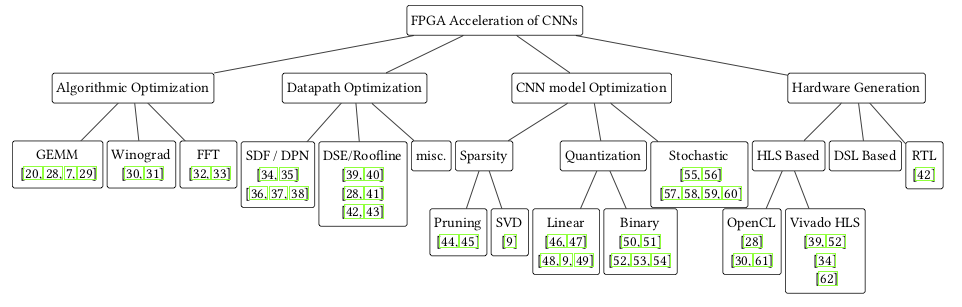
\includegraphics[width=\textwidth]{Figures/InferenceOpt.png}
% 	\caption[Inference Optimisations]{Methods to accelerate an FPGA implementation \cite{Abdelouahab2018}}
% 	\label{fig:InferenceOpt}
% \end{figure}


% QUANTISED LENET THROUGH NETRON
% \begin{figure}[htbp]
% 	\centering
% 		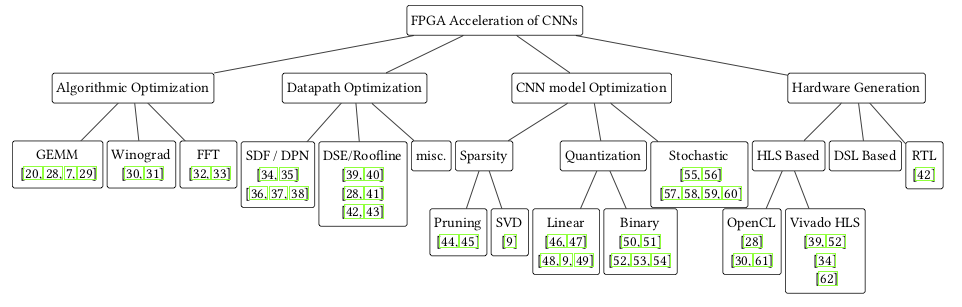
\includegraphics[width=\textwidth]{Figures/InferenceOpt.png}
% 	\caption[Inference Optimisations]{Methods to accelerate an FPGA implementation \cite{Abdelouahab2018}}
% 	\label{fig:InferenceOpt}
% \end{figure}

%-------------------------
%	SUBSECTION 6.2.3 - FINN
%-------------------------

\subsection{FINN}

% FINN WHOLE FLOW
% \begin{figure}[htbp]
% 	\centering
% 		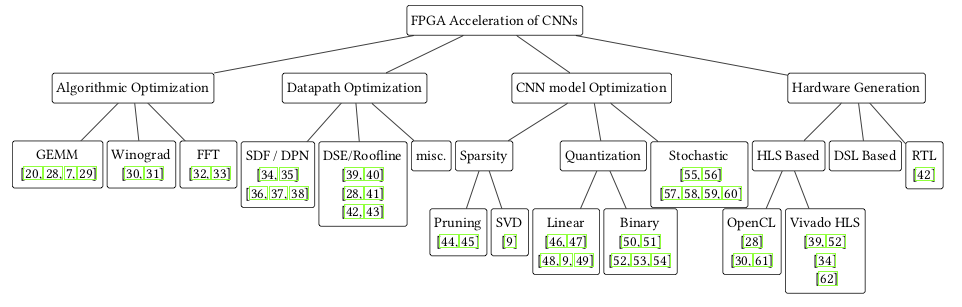
\includegraphics[width=\textwidth]{Figures/InferenceOpt.png}
% 	\caption[Inference Optimisations]{Methods to accelerate an FPGA implementation \cite{Abdelouahab2018}}
% 	\label{fig:InferenceOpt}
% \end{figure}

The last piece of the workflow is \emph{FINN}, described by Xilinx as allowing \guille{Fast, Scalable Quantized Neural Network Inference on FPGAs}. The \emph{FINN} compiler goes through three major steps to be able to port a neural network. First, \emph{Network Preparation} where \emph{FINN} uses different transformations on the \emph{ONNX} graph to simplify it or make it more convenient for the next steps. Then, \emph{IP Generation} where the \emph{Vivado} tool is called to generate a network of HLS layers with one IP block per layer and finally stitches all the blocks together. Finally, the network is deployed on an FPGA with a \emph{PYNQ} shell, an FPGA utility providing a Python environment on an FPGA. This deployment is made possible by creating a project and driver then transferring it on the board along with the bitfile.

% IMAGE OF FINN WHOLE FLOW
% \begin{figure}[htbp]
% 	\centering
% 		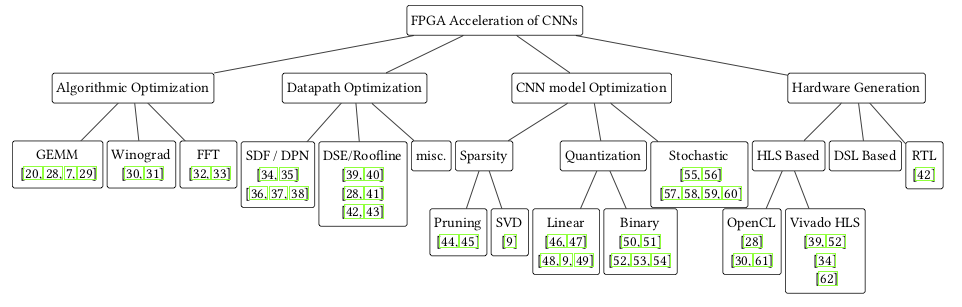
\includegraphics[width=\textwidth]{Figures/InferenceOpt.png}
% 	\caption[Inference Optimisations]{Methods to accelerate an FPGA implementation \cite{Abdelouahab2018}}
% 	\label{fig:InferenceOpt}
% \end{figure}

The network preparation part is the one involving several transformations in the structure of the neural network graph. The transformations are separated in three categories: tidy-up,
 streamlining, HLS conversion and dataflow partition. All the different transformations, whether they are used for tidy-up or synthesis purposes, are applied on a \texttt{ModelWrapper}.

\emph{Tidy-up Transformations} consist of renaming the nodes so they have unique names, checking the data type and shapes of the tensors used. Example of them are \texttt{GiveReadableTensorNames}, \texttt{GiveUniqueNodeNames} or \texttt{InferShapes}.

\emph{Streamline Transformations} consist of a way to remove floating-point operations from the graph. The streamlining process itself contains three steps:
\begin{itemize}
  \item \textbf{Successive Thresholding}: Given a set of threshold values, the successive thresholding function maps any real number $x$ to an integer corresponding to the number of thresholds $x$ is greater or equal to. This way, any uniform quantifier can be expressed as successive thresholding followed by a linear transformation: $Q(x) = a*T(x) + b$.
  \item \textbf{Collapsing Linear Transformation}: All \emph{floating point} linear operations are positioned between the quantised matrix operation and the activation quantisation. Any sequence of linear transformation can be collapsed in a single linear transformation.
  \item \textbf{Absorbing into Thresholds} :Updating the threshold values with the changes in the linear transformations removes any linear transformation from the graph.
\end{itemize}

The \texttt{Streamline} transformation class is implemented as presented on \emph{Figure} \ref{fig:FINNStreamline}.

\begin{figure}[htbp]
\centering
\begin{lstlisting}[language=Python]
class Streamline(Transformation):
  """Apply the streamlining transform, see arXiv:1709.04060."""

  def apply(self, model):
    streamline_transformations = [
      ConvertSubToAdd(),
      ConvertDivToMul(),
      BatchNormToAffine(),
      ConvertSignToThres(),
      MoveAddPastMul(),
      MoveScalarAddPastMatMul(),
      MoveScalarAddPastConv(),
      MoveScalarMulPastMatMul(),
      MoveScalarMulPastConv(),
      MoveAddPastMul(),
      CollapseRepeatedAdd(),
      CollapseRepeatedMul(),
      AbsorbAddIntoMultiThreshold(),
      FactorOutMulSignMagnitude(),
      AbsorbMulIntoMultiThreshold(),
      Absorb1BitMulIntoMatMul(),
      Absorb1BitMulIntoConv(),
      RoundAndClipThresholds(),
    ]
    for trn in streamline_transformations:
      model = model.transform(trn)
      model = model.transform(GiveUniqueNodeNames())
      model = model.transform(GiveReadableTensorNames())
      model = model.transform(InferDataTypes())
    return (model, False)
\end{lstlisting}
\caption[FINNStreamline]{FINN Streamline process as proposed in }
	\label{fig:FINNStreamline}
\end{figure}


%-------------------------------------------
%	SUBSECTION 6.2.4 - Benchmark as extension
%-------------------------------------------

\subsection{Benchmark as Extension}

%----------------------------------------------------------------------------------------
%	SECTION 6.3 - Methodology and Setup
%----------------------------------------------------------------------------------------

\section{Methodology and Setup}

%-----------------------------------
%	SUBSECTION 6.3.1 - Motivations
%-----------------------------------

\subsection{Experiments}

%--------------------------------------
%	SUBSECTION 6.3.2 - Training
%--------------------------------------

\subsection{Training}

%--------------------------------------
%	SUBSECTION 6.3.3 - Deployment
%--------------------------------------

\subsection{Deployment}
